\documentclass[a4paper,10pt]{article}
%\documentclass[a4paper,10pt]{scrartcl}

\usepackage[utf8]{inputenc}
\usepackage{amsmath}
\usepackage{listings}
\usepackage{hyperref}
\usepackage{catoptions}
\usepackage[margin=1in]{geometry}
\usepackage{color}
\usepackage{soul}
\usepackage{float}
\usepackage{framed}
\usepackage[sc]{mathpazo}
\linespread{1.20}         % Palatino needs more leading (space between lines)
\usepackage[T1]{fontenc}
\usepackage{microtype}
\usepackage{enumerate}
\usepackage{courier}
\usepackage{graphicx}
\usepackage{newclude}

\newcommand{\authorbd}{Bas Dado (4033736)}
\newcommand{\authoroh}{Olivier Hokke (1352679)}
\newcommand{\authortr}{Tom Runia (1517996)}
\newcommand{\authoras}{Arnold Schutter (4260724)}
\newcommand{\authortv}{Tom Viering (4333055)}
\newcommand{\maintitle}{IN4010: Negotiation Project}
\newcommand{\subtitle}{Group 7 - BOAconstructor}

\title{\maintitle\\\subtitle}
\author{\authorbd\\\authoroh\\\authortr\\\authoras\\\authortv}
\date{\today}

\pdfinfo{%
  /Title    (\maintitle - \subtitle)
  /Author   (\authorbd, \authoroh, \authortr, \authoras, \authortv)
  /Creator  (\authorbd, \authoroh, \authortr, \authoras, \authortv)
  /Producer (\authorbd, \authoroh, \authortr, \authoras, \authortv)
  /Subject  (Automated Negotiation)
  /Keywords (Automated Negotiation, Genius, Bidding Strategy, Acceptance Strategy, Opponent Model, Opponent Model Strategy)
}

% Settings for hyperref package (e.g. wat \autoref en \nameref moeten doen)
\hypersetup{
  colorlinks  = true,
  linkcolor   = [rgb]{0.1,0.1,0.5},
  citecolor   = [rgb]{0.5,0.1,0.1},
  filecolor   = [rgb]{0.1,0.5,0.5},
  urlcolor    = [rgb]{0.1,0.1,0.7}
}

% Adds the command "\Autoref" to make it possible to use a capital in the referenced object name
\makeatletter
\def\figureautorefname{figure}
\def\tableautorefname{table}
\def\Autoref#1{%
  \begingroup
  \edef\reserved@a{\cpttrimspaces{#1}}%
  \ifcsndefTF{r@#1}{%
    \xaftercsname{\expandafter\testreftype\@fourthoffive}
      {r@\reserved@a}.\\{#1}%
  }{%
    \ref{#1}%
  }%
  \endgroup
}
\def\testreftype#1.#2\\#3{%
  \ifcsndefTF{#1autorefname}{%
    \def\reserved@a##1##2\@nil{%
      \uppercase{\def\ref@name{##1}}%
      \csn@edef{#1autorefname}{\ref@name##2}%
      \autoref{#3}%
    }%
    \reserved@a#1\@nil
  }{%
    \autoref{#3}%
  }%
}
\makeatother

% Settings for listings of java code
\definecolor{mygreen}{rgb}{0,0.6,0}
\definecolor{light-gray}{gray}{0.95}
\lstset{basicstyle=\footnotesize\ttfamily,breaklines=true,language=Java}
\lstset{frame=single,commentstyle=\color{mygreen},keywordstyle=\color{blue}}
\lstset{aboveskip=0.5cm,belowskip=0.3cm}
\lstset{backgroundcolor=\color{light-gray}}

% Define the todo command
\newcommand{\todo}[1] {\hl{TODO: #1}}
\setlength{\parindent}{0cm}

\begin{document}
\maketitle

\section{Introduction}
\label{sec:introduction}
\include*{introduction}

\newpage
\tableofcontents
\newpage


\section{Exercises}
\label{sec:exercises}

\subsection{Party domain analysis}

\subsubsection{Bidding space and pareto frontier}

In this subsection we analyse the party domain and compute the Pareto frontier.
The party domain has 6 issues: food (4 options), drinks (4 options), 
locations (4 options), invitations (4 options), music (3 options), cleanup (4 options).
This results in $4 \times 4 \times 4 \times 4 \times 3 \times 4 = 3072$ outcomes.
We took the preference profile of user 10 and 15 of the party domain,
we compute the outcome space and the pareto frontier and plot this in the figure below:

%\begin{figure}[ht]
\begin{center}
 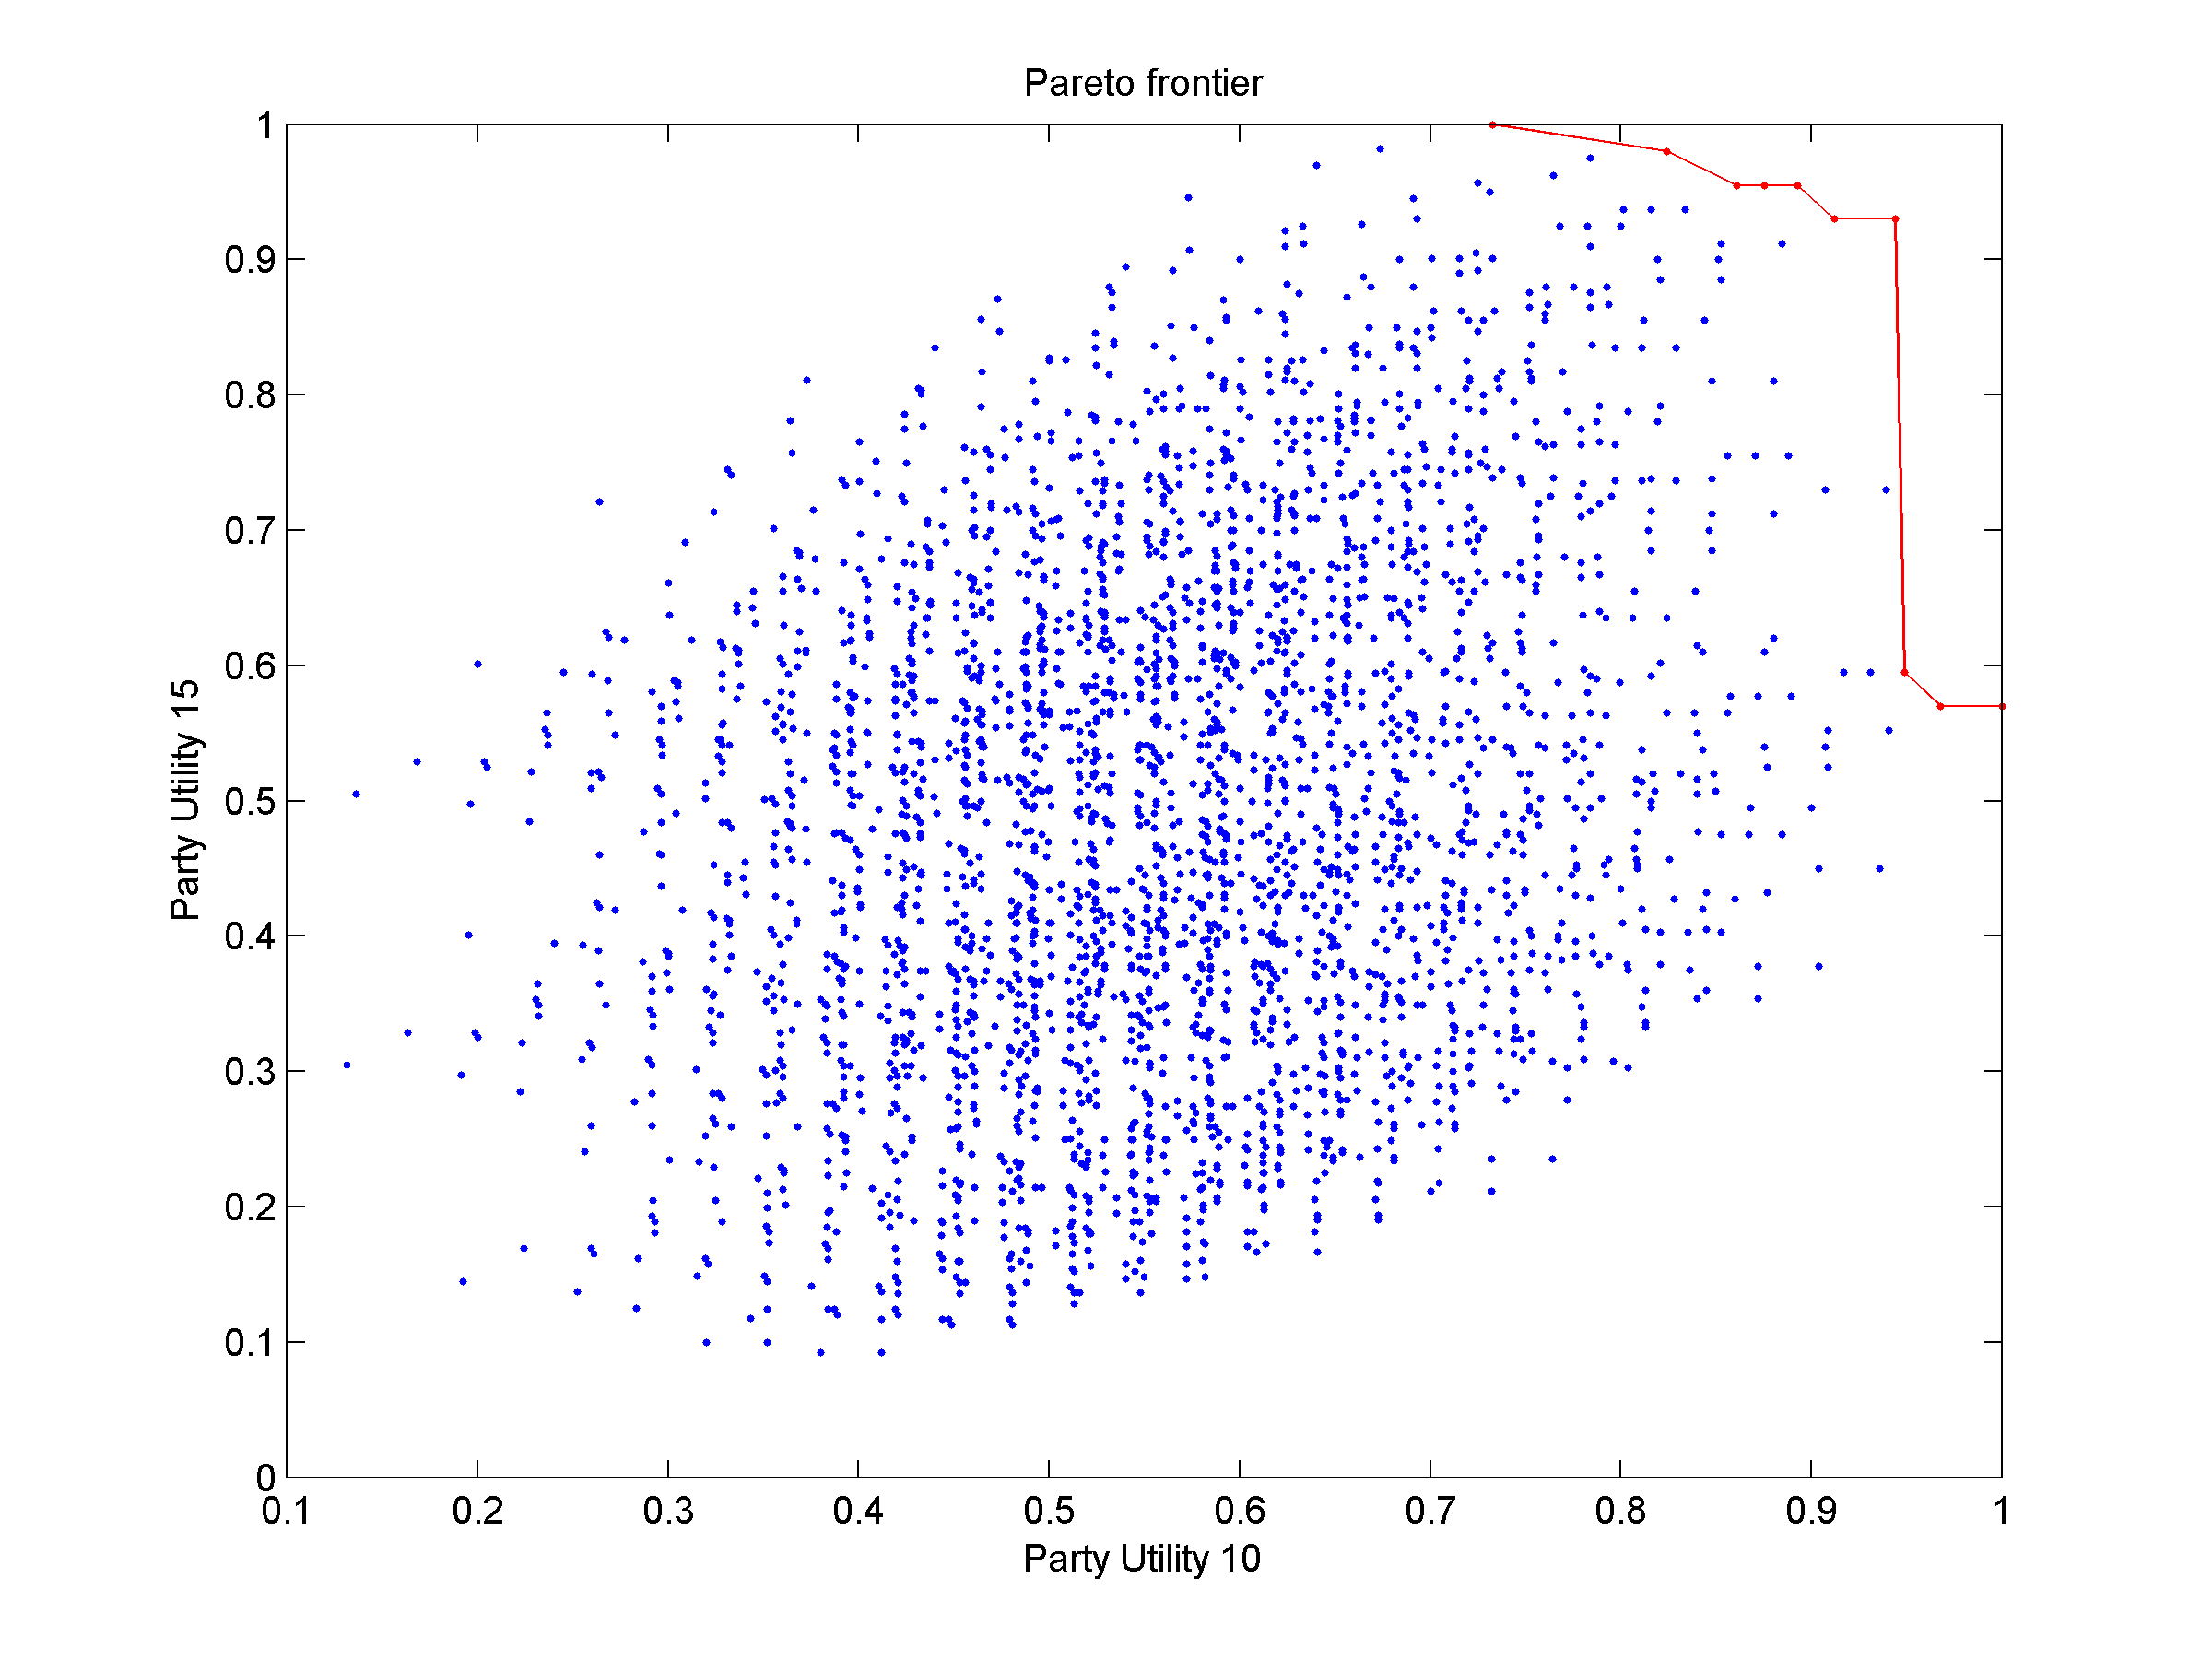
\includegraphics[width=0.6\textwidth]{pareto.png}
% \caption{The pareto optimal frontier is displayed with a red line in this figure.}
% \label{fig:pareto} 
\end{center}
%\end{figure}

\subsubsection{Analyse simple opponents}

Finally, we perform two negotiation sessions: we play with the agent SimpleAgent against
itself, and we play Boulware vs Conceder and explain the outcome. 

When we play simple agent against itself, we notice the behaviour is quite random.
This is explained by the code: it always offers a random bid higher than a certain threshold,
by default this threshold is zero. Therefore it performs a random walk through the 
bidding space. It's acceptance strategy is as follows: it calculates a probability for each bid, the higher the bid, the higher the probability. If the deadline is getting closer it will accept all bids with higher probability. It will however never accept bids with a utility of zero. The equation that determines the 
probability of acceptance is:

\begin{equation}
P = \frac{u - 2ut + 2(-1 + t + \sqrt{((-1 + t)^2 + u(-1 + 2t)})}{-1 + 2t}
\end{equation}

Where $P$ denotes the chance of acceptance, $u$ denotes the utility of the bid and $t$ denotes the time in a range of $[0,1]$.

Because of this behaviour we found the average utility playing against itself is around $0.68$, and the
time needed to reach an agreement was very short: $0.03$ (averaged
over 20 negotiations on the party domain).
This is quite logical, since both sides offer random bids, it is the
case quite soon that either bid has a high probability of acceptance for the opposing party.
When this agent negotiates with other agents, it performs badly, because
it offers random bids. Smart agents will accept good offers and deny other offers,
and because of this the obtained utility for the simple agent will be quite low.
We confirm this by letting simple agent play against boulware. In these tests the simple agent obtains 
an average utility of $0.6$ while the boulware agent scores on average $1.0$.

Finally, we play with the boulware agent against the conceder agent. A typical negotiation trace is displayed below:

%\begin{figure}[ht]
\begin{center}
 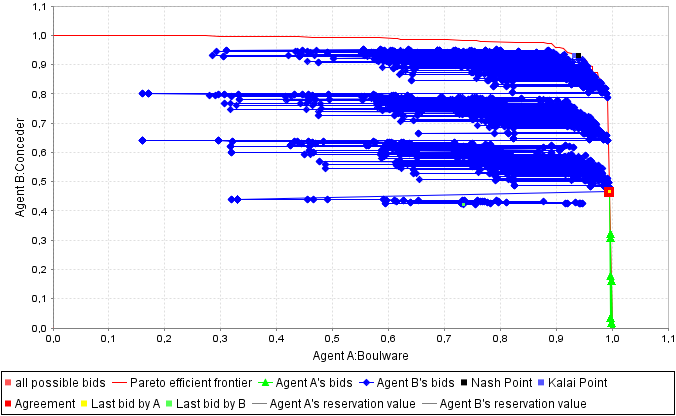
\includegraphics[width=0.6\textwidth]{traceConcederBoulware.png}
% \caption{The pareto optimal frontier is displayed with a red line in this figure.}
% \label{fig:pareto} 
\end{center}
%\end{figure}
In the figure, the green and blue lines are the bidding-traces for respectively the boulware and the conceder agent. The boulware agent chooses the best bid for itself, and keeps offering this bid. This agent
only concedes at the very last moments before the deadline. The conceder agent on the other hand
starts conceding directly and keeps on conceding every new bid. We ran simulations on the party domain using these agents. Averaging over 20 negotiations the conceder reached an utility of $0.67$ and
boulware $0.99$. 
 
\subsection{PEAS Description}

The first step in designing an agent is to specify the environment as fully as possible. In order to do this we specify the PEAS description which lists the following aspects of the environment: \emph{Performance}, \emph{Environment}, \emph{Actuators} and \emph{Sensors}. This measure is extensively discussed in Russel and Norvig \cite{russel-norvig}, so we adapt their notation.

\begin{table}[H]
    \begin{tabular}{|p{1.8cm}|p{3cm}|p{3cm}|p{3cm}|p{3cm}|}
    \hline
    \textbf{Agent} & \textbf{Performance \mbox{Measure}} & \textbf{Environment} & \textbf{Actuators} & \textbf{Sensors} \\
    \hline
    BOA Agent & Own $($versus \mbox{opponents}$)$ discounted final utility & Negotiation space defined by Genius, \mbox{Opponents} & New bid offering, \mbox{Accepting/rejecting} offers & Java classes that return the bidding history of the \mbox{opponent} agent \\
    \hline
    \end{tabular}
    
    \caption{PEAS description for our negotiation agent \label{table:peas-description}}
\end{table}

Table~\ref{table:peas-description} displays the PEAS description for our agent. We will briefly discuss each of the descriptions. First the \emph{environment} our agent operates in, this is the negotiation space as defined by Genius. \todo{Check the PEAS description I came up with and finish the additional description} 

\subsection{BOA Framework}

Most negotiation agents consist of three components: \emph{Bidding strategy}, \emph{Opponent model}, \emph{Acceptance strategy}. Together these three components form the \emph{BOA framework}. As discussed by Baarslag et al., the advantages of separating the components using this framework are threefold \cite{baarslag2012decoupling}. In designing our negotiation agent the most useful advantage was the fact that it allows for easily changing individual components and analyze the interaction between the components. Below we provide a small description for the three required components.

\begin{description}
  \item[Bidding Strategy] \hfill \\
  The bidding strategy is arguably the most important component. Its goal is to determine the next bid that is offered to the opponent. In determining the next bid the agent can interact with the opponent model to provide a suitable offer. Sometimes the negotiation sessions is split up in multiple phases and each of the phases uses a different bidding strategy.

  \item[Opponent Model] \hfill \\
  Learning the opponents behaviour is essential in a good negotiation session. It allows for adapting to the way the other party provides its bids. In practice this works by estimating the opponents \emph{preference profile}, which is usually done by adapting \emph{Bayesian modelling} or \emph{frequency analysis}.

  \item[Acceptance Strategy] \hfill \\
  Negotiation sessions ideally end by reaching an agreement. The acceptance strategy decides whether the opponents offer should be accepted. A broad variety of acceptance strategies is available reaching from postponing acceptance until the last step and aiming at fast decisions.

\end{description}

\section{Strategy}
\label{sec:strategy}

\subsection{Bidding Strategy}
\label{sec:strategyBS}
\include*{strategy_bidding_strategy}

\subsection{Opponent Model}
\label{sec:strategyOM}
\include*{strategy_opponent_model}

\subsection{Acceptance Strategy}
\label{sec:strategyAS}
\include*{strategy_acceptance_strategy}

\subsection{Opponent Strategy Model}
\label{sec:strategyOMS}
\include*{strategy_opponent_strategy_model}

\section{Testing \& Performance}
\label{sec:performance}
\include*{testing_and_performance}


\section{Conclusion}
\label{sec:conclusion}
\include*{conclusion}

\bibliography{negotiation_final_report}
\bibliographystyle{plain}

\end{document}
